\newpage
\subsection{Admin Page}
The admin page is divided into four sections: “dashboard”, “List of Students”, “Teachers” and “Student Request”. The main area of the dashboard section contains the total number of users and courses details. The all requests form registered students at the system  are located at the “Student Request” section and admin can give the access to the portal or reject the request.\\

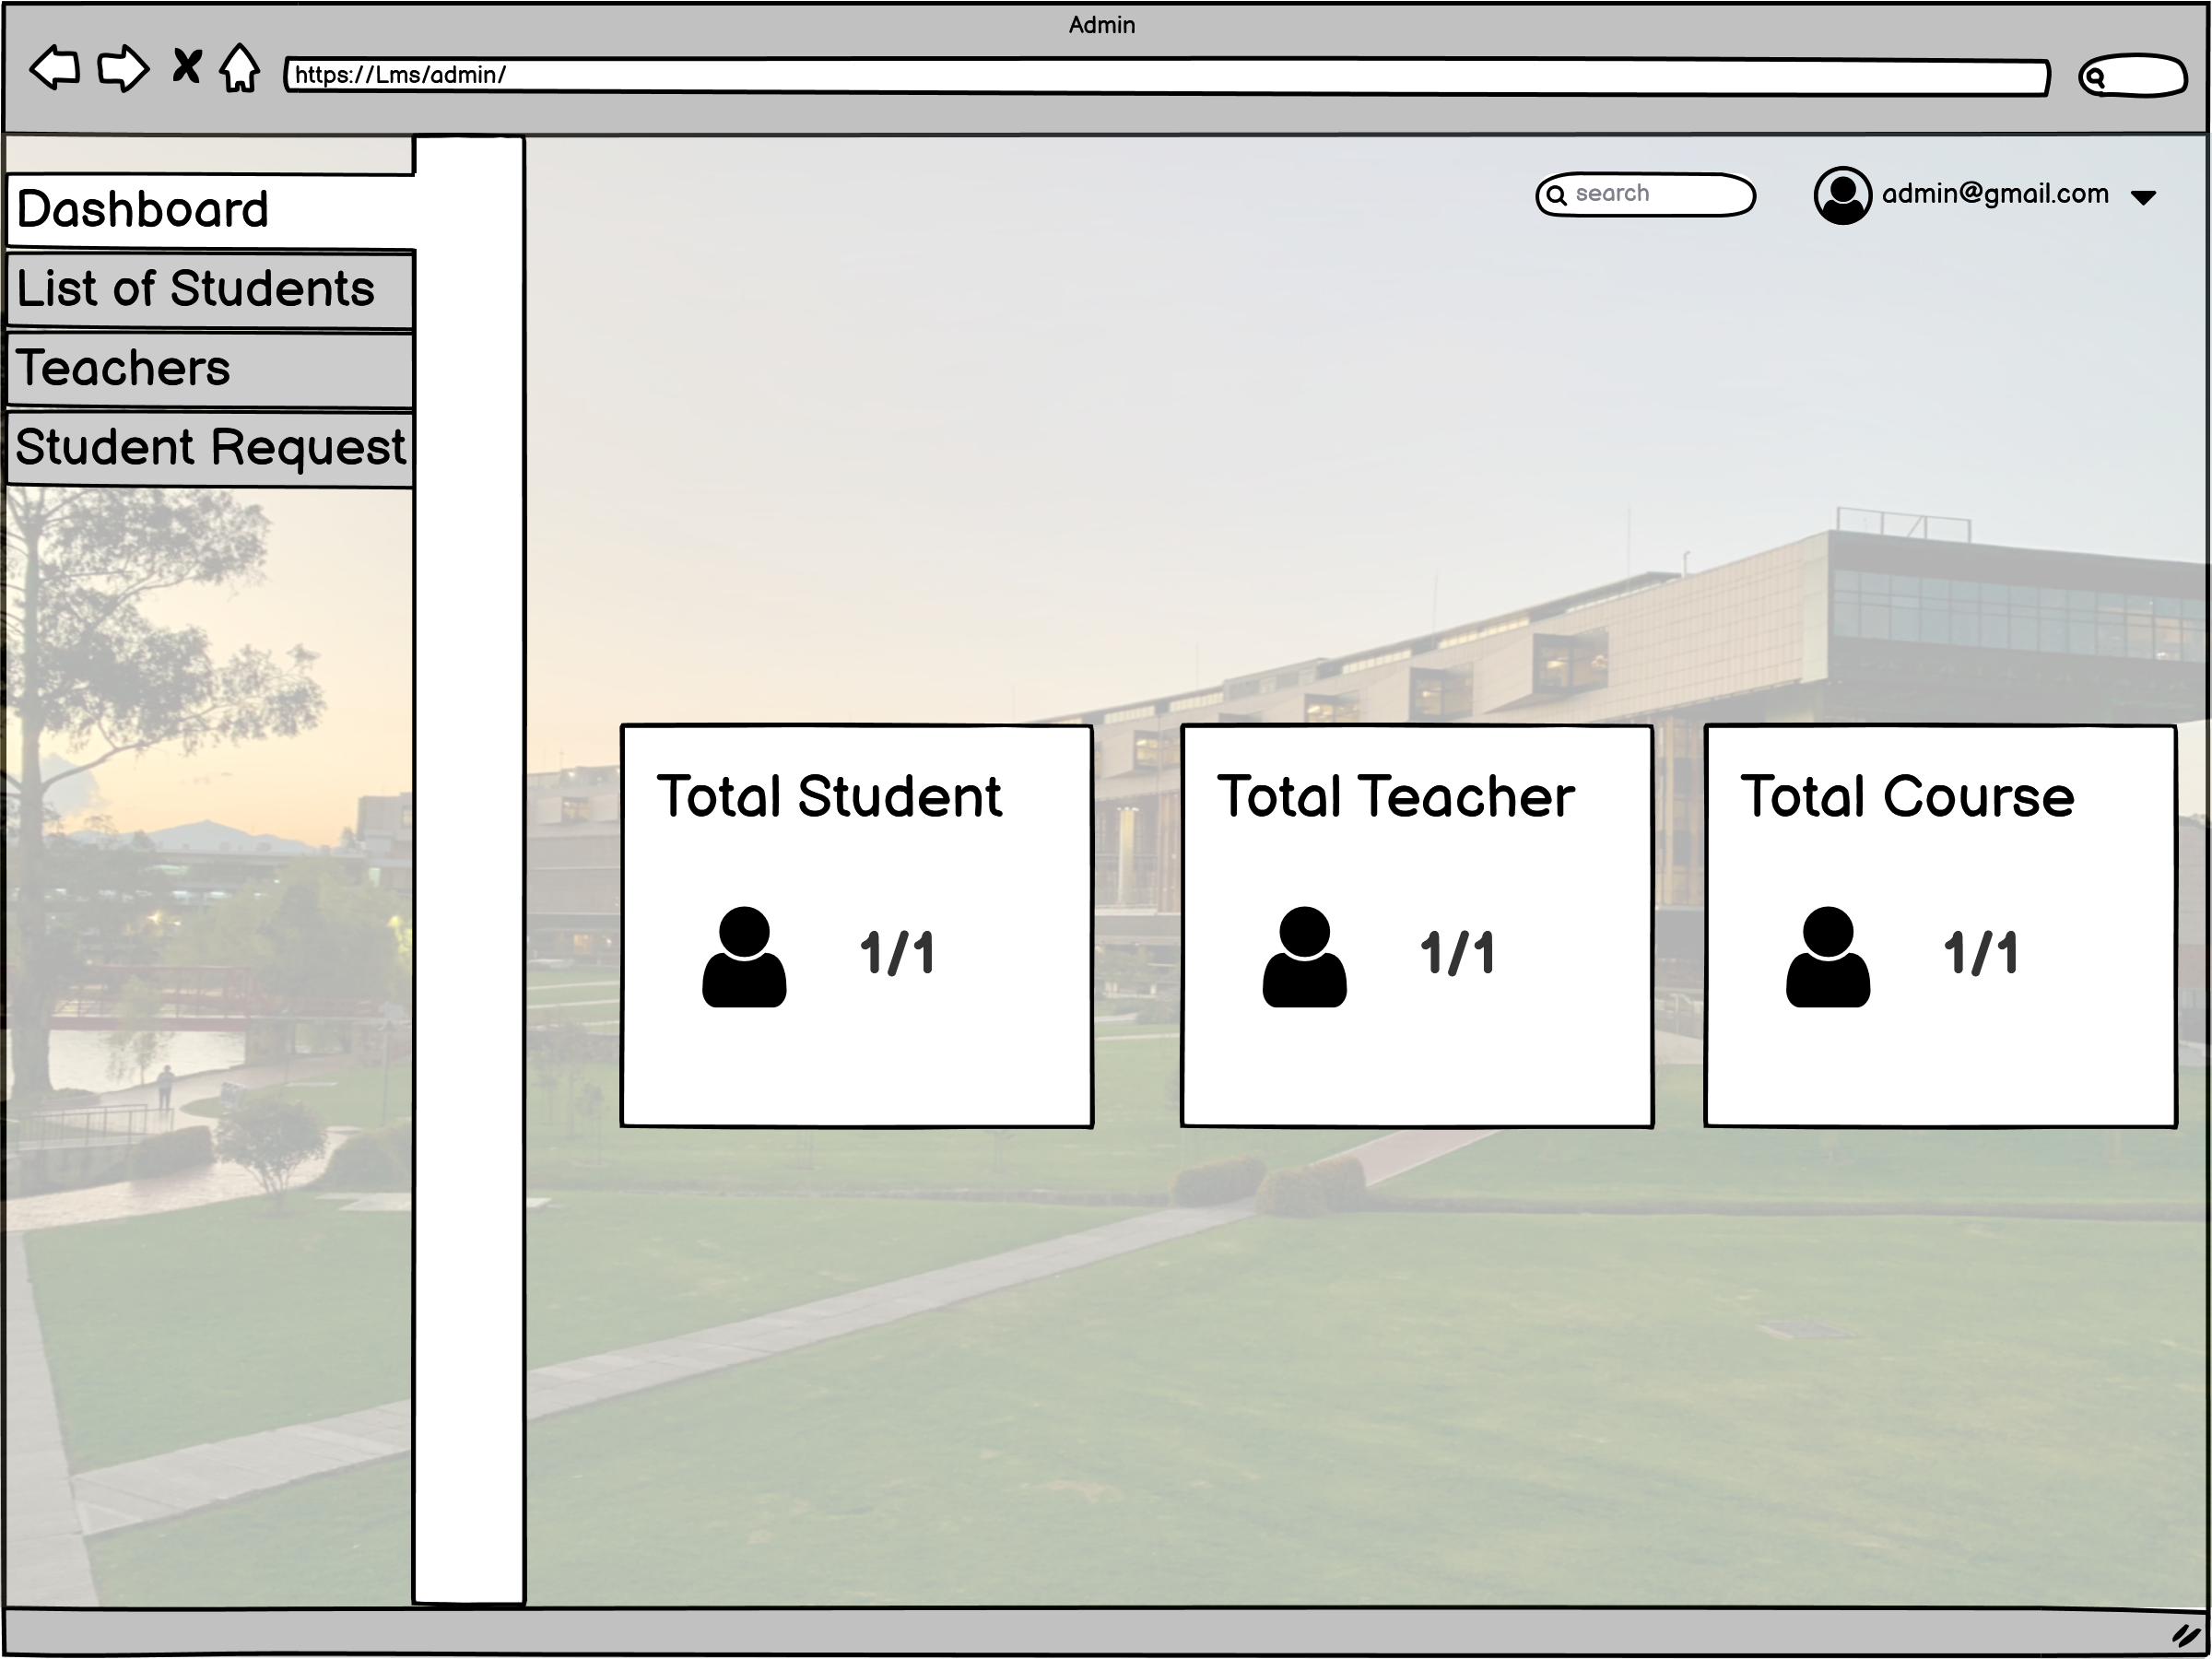
\includegraphics[width=\columnwidth]{images/Admin Page.png}\\
\newpage
The admin page allows to register new teachers going to “Teachers” section. It contains a table  with all the information about each teacher and also there is a “Modify” column where admin can update or delete data.  Clicking on the button “update” admin updates the user details, or the button “delete” admin deletes the user from the database, revoking their possibility to login and therefore to access the courses. Clicking to the “add teacher” button the admin is going to registration page for adding a new teacher to the system.\\ 

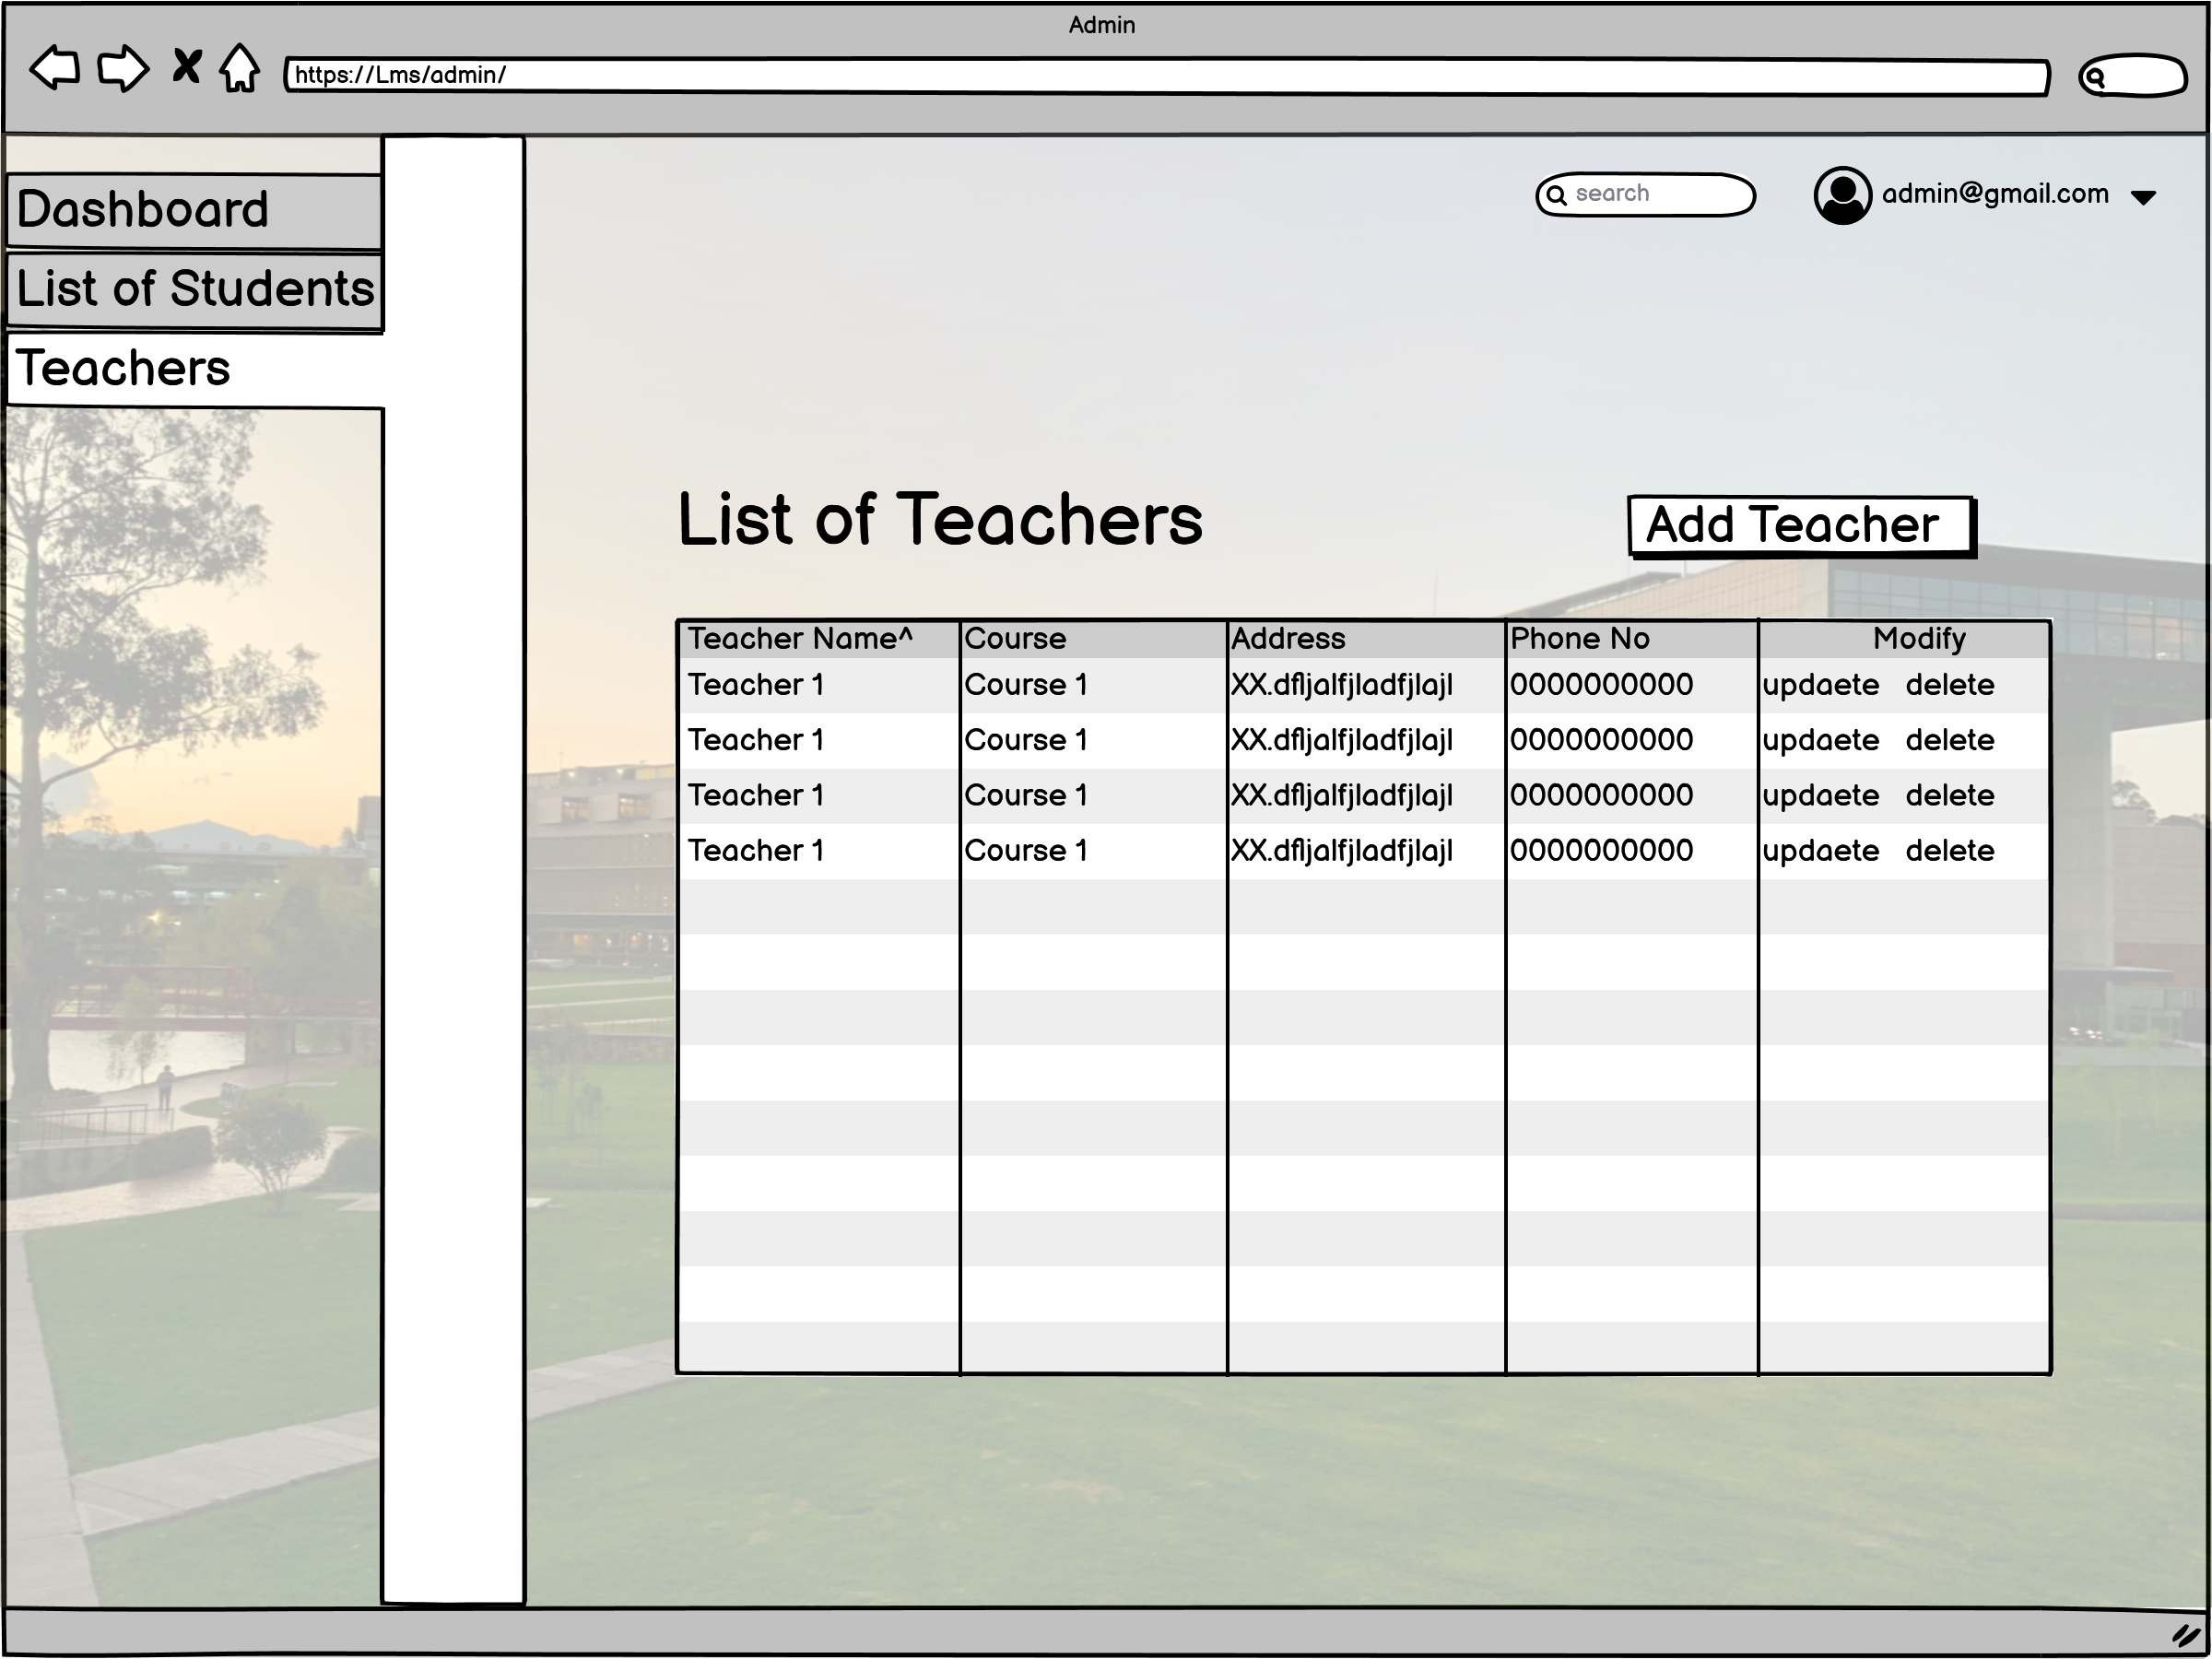
\includegraphics[width=\columnwidth]{images/Teachers.png}\\
\newpage
The Teacher registration page contains a form for manual filling in the name, e-mail, address and password. The Gender field gives the option to choose between three variants and at the Course field the subject can be selected from the database. After the form is filled in the admin submits it by clicking the Register button.\\

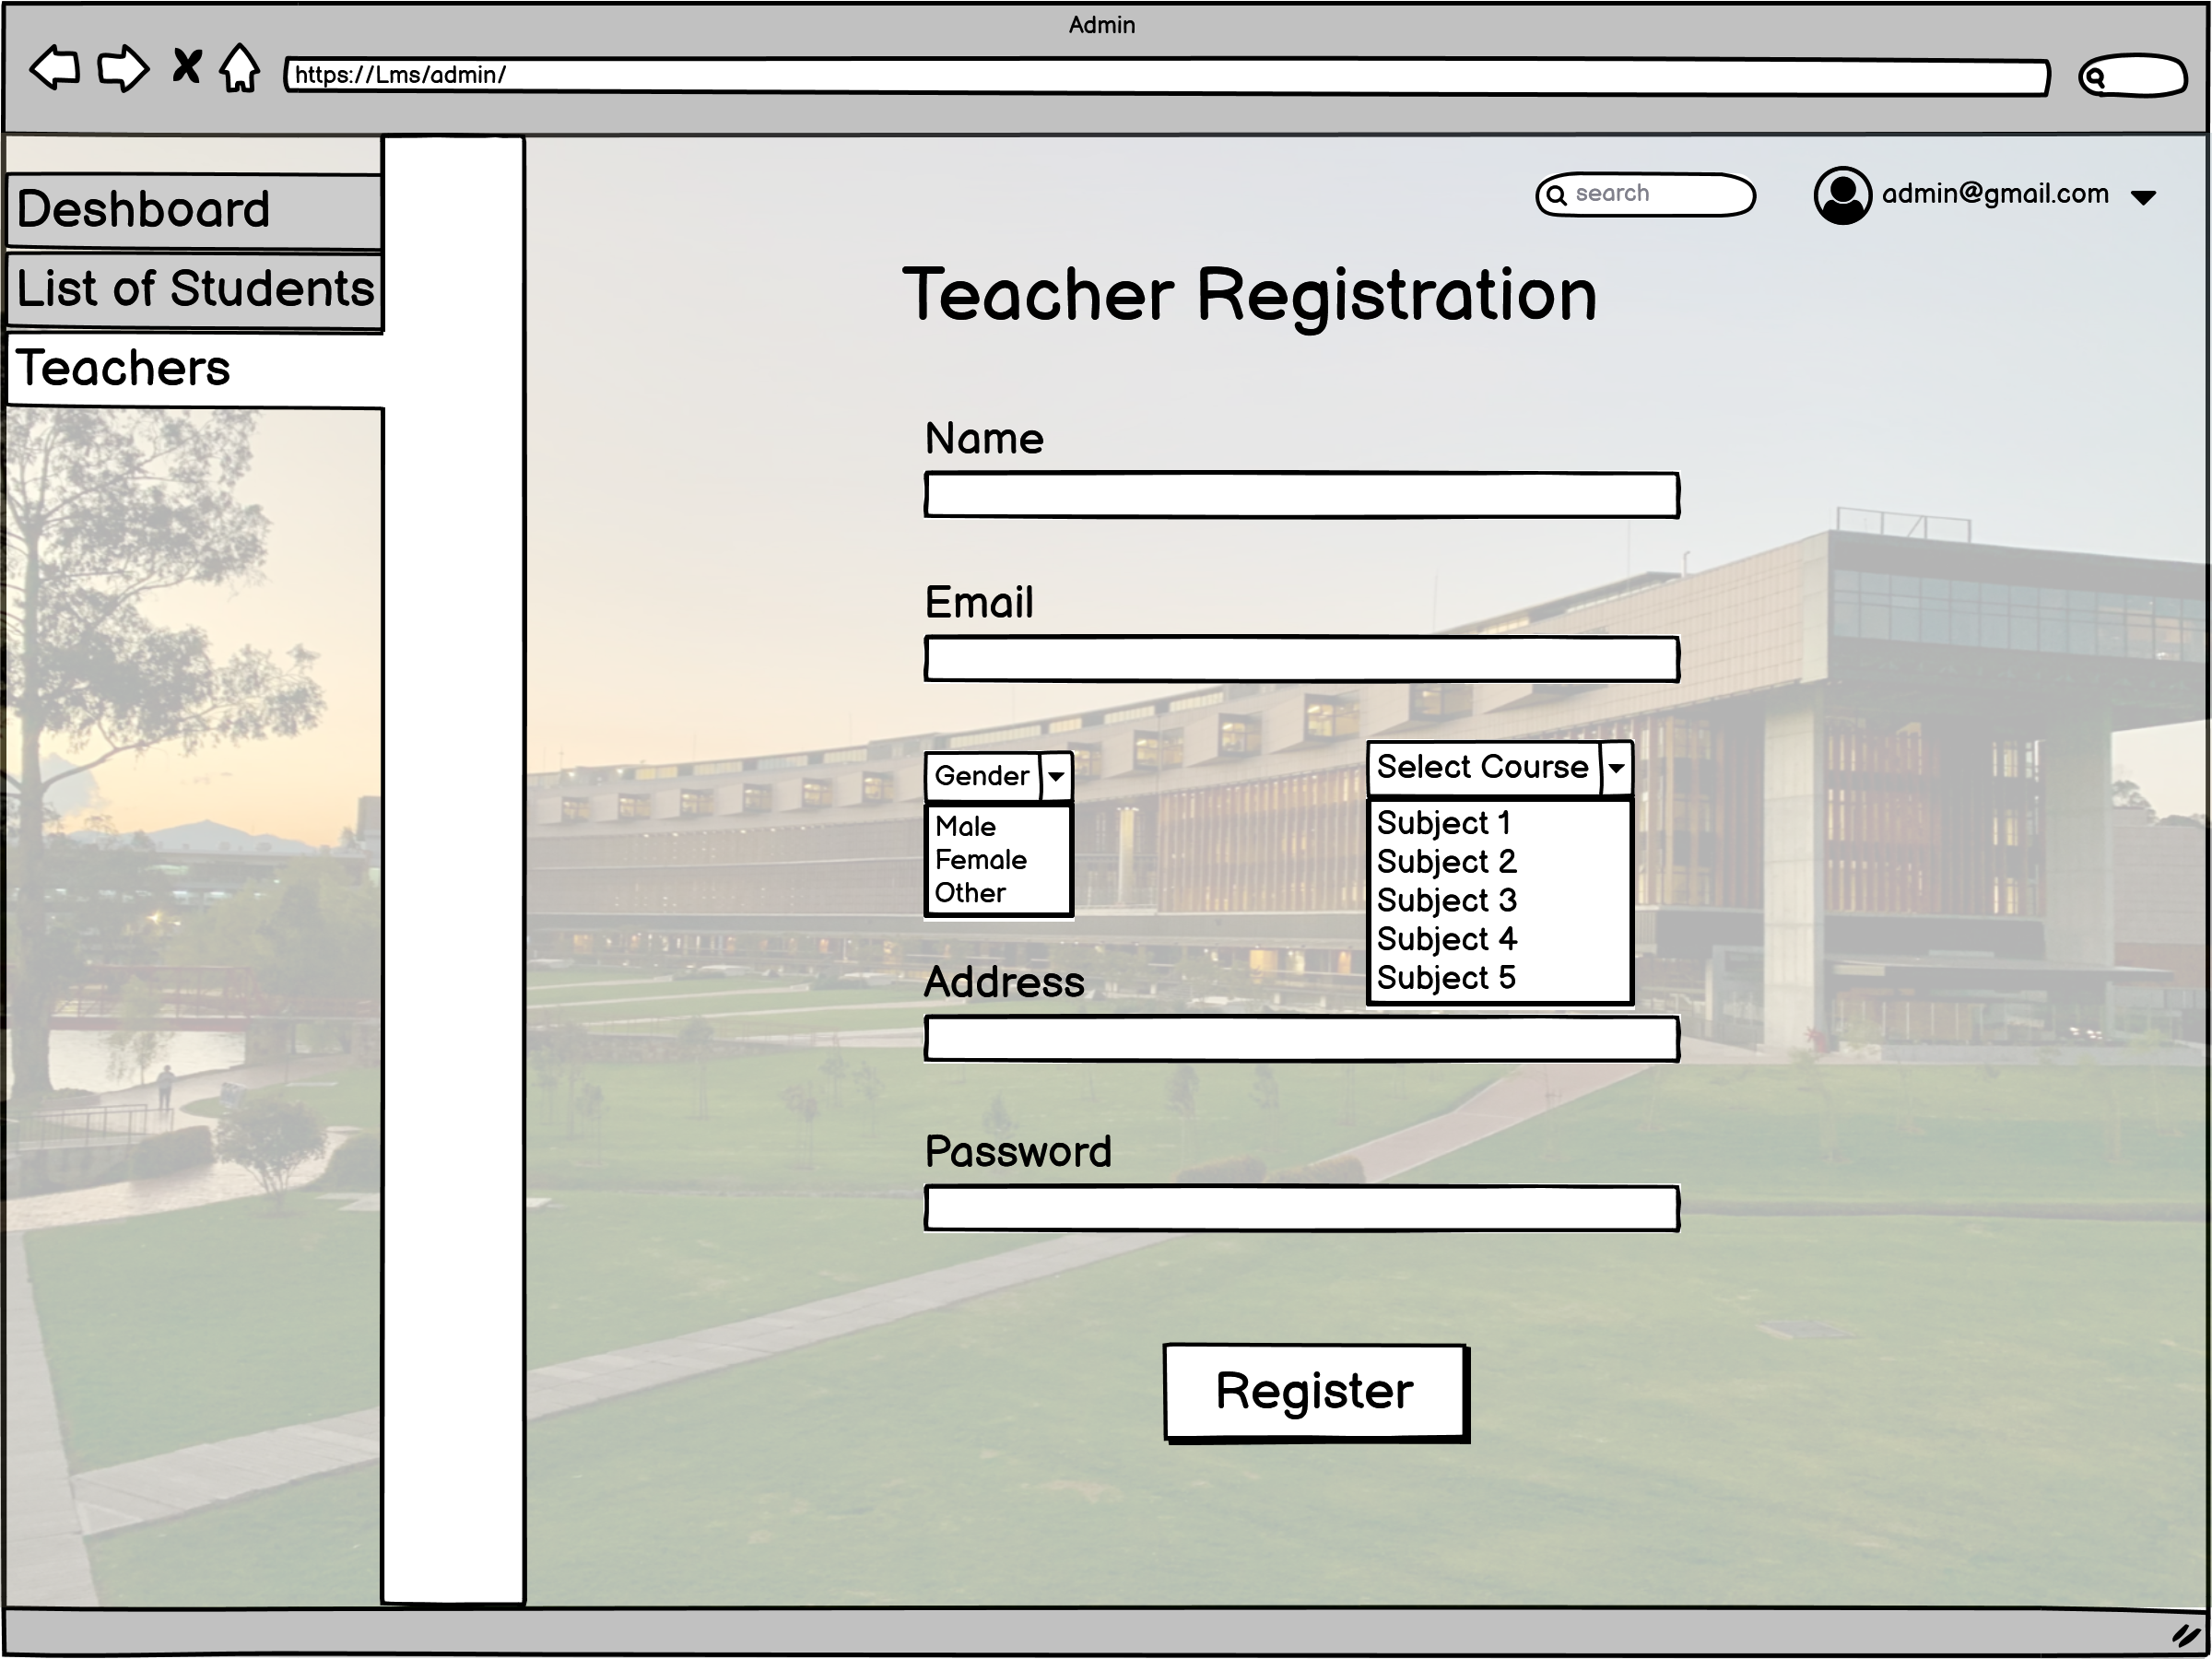
\includegraphics[width=\columnwidth]{images/TeacherRegistration.png}\\
\newpage
The “List of Students” section contains a table  with all the information about each student and also there is a “Modify” column where admin can update or delete data.  Clicking on the button “update” admin updates the user details, or the button “delete” admin deletes the user from the database, revoking their possibility to login and therefore to access the courses.\\


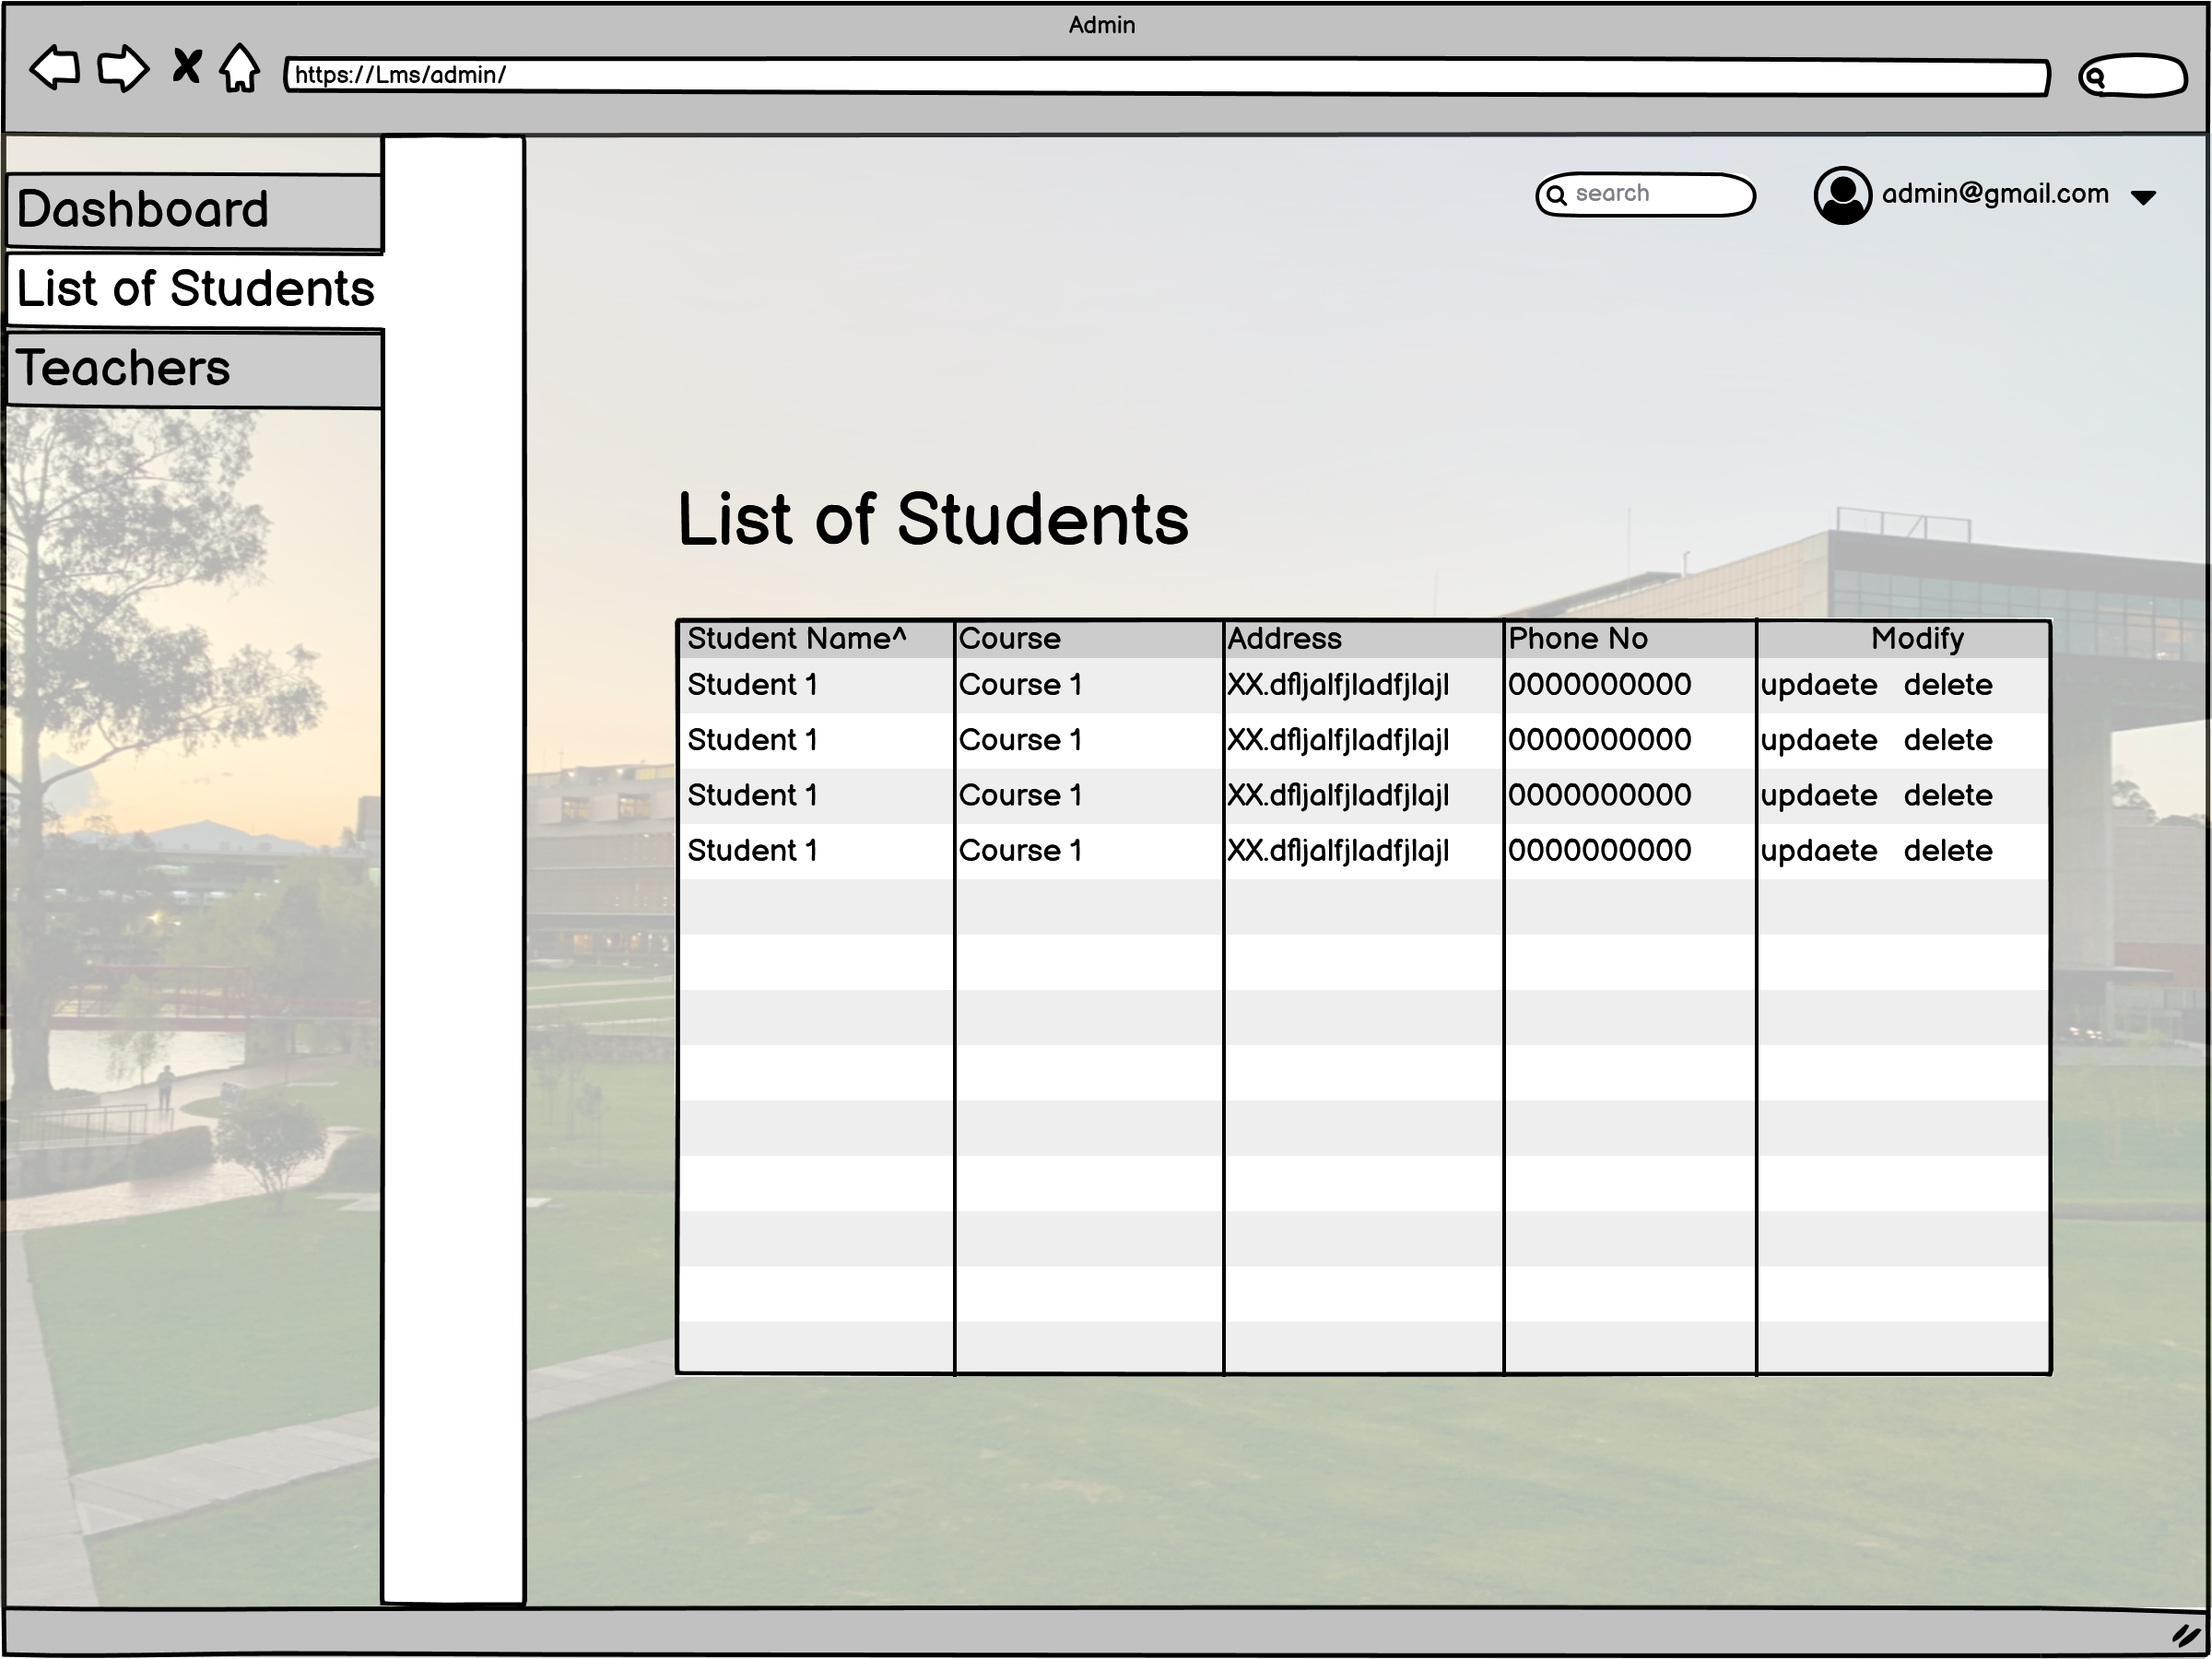
\includegraphics[width=\columnwidth]{images/List of Students.png}